\documentclass[conference]{IEEEtran}
\IEEEoverridecommandlockouts

\usepackage{cite}
\usepackage{amsmath,amssymb}
\usepackage{graphicx}
\graphicspath{{../assets/}}
\usepackage{booktabs}
\usepackage{array}
\usepackage{tabularx}
\usepackage{dblfloatfix}
\usepackage{url}
\usepackage[hidelinks]{hyperref}

\title{Semantic-Aware Dynamic 3D Gaussian Splatting with SAM 2--CLIP Distillation and Object-Level Editing}

\author{\IEEEauthorblockN{Uthkarsh Sai, Akhil Reddy, Tenisha Akhila, Jagapathi Naidu, and Jeevita Bhupati}
\IEEEauthorblockA{Group 08, Computer Vision Course Project\\Amrita Vishwa Vidyapeetham, India}}

\begin{document}
\maketitle

\begin{abstract}
Dynamic 3D Gaussian Splatting (4D-GS) represents a time-varying scene with explicit Gaussians and a learned deformation field, enabling efficient novel-view rendering. Appearance and motion alone, however, do not provide explicit object or part identity for semantic selection and editing. This project investigates a prototype extension that combines a 4D-GS code path with per-frame semantic supervision derived from Segment Anything Model 2 (SAM 2) masks and Contrastive Language--Image Pretraining (CLIP) features. The repository also contains a separate, static multi-view semantic-transfer pathway that projects Gaussian centers into calibrated camera images and aggregates mask labels by voting. A Gaussian editing prototype supports class-conditioned selection and localized appearance or position changes. We describe these components, their interfaces, and their limitations. The available checked-in evaluation path supports pixel-space label-map IoU when predictions and ground-truth labels are supplied; it does not establish 3D semantic accuracy, temporal consistency, photometric quality, frame rate, or editing quality. Consequently, this report makes no quantitative performance claim and presents the work as an implementation prototype pending reproducible end-to-end experiments.
\end{abstract}

\begin{IEEEkeywords}
4D Gaussian Splatting, dynamic scene reconstruction, semantic distillation, SAM 2, CLIP, multi-view projection, Gaussian editing.
\end{IEEEkeywords}

\section{Introduction}
Three-dimensional Gaussian Splatting (3DGS) represents a scene using explicit anisotropic Gaussians and differentiable rasterization, offering high-quality rendering with an efficient optimization and display pipeline~\cite{kerbl2023gs}. Dynamic scenes require the representation to account for motion over time. 4D-GS augments canonical Gaussians with a time-conditioned deformation model and spatial-temporal features, including HexPlane representations~\cite{wu20244dgs,wang2023hexplane}. These methods primarily model geometry, motion, and appearance; those quantities do not by themselves provide reliable object identity or text-queryable semantic attributes.

This project explores semantic supervision and object-level interaction for dynamic Gaussian scenes. The dynamic pathway uses 2D masks and image-language features as training targets for semantic attributes associated with Gaussians. In addition, the repository includes a geometric semantic-transfer pipeline for static 3D Gaussian clouds: it projects Gaussian centers into calibrated views, samples 2D masks, and aggregates observations across views. These pathways address related but distinct settings and should not be interpreted as a single validated end-to-end system.

The contributions of this project are engineering and methodological prototypes:
\begin{itemize}
    \item A code path for attaching learnable semantic attributes to the 4D-GS Gaussian model and applying semantic supervision during fine-stage training.
    \item A SAM 2--CLIP preprocessing path that converts image masks and text prompts into per-frame label maps and dense feature maps.
    \item A separate static-scene projection and multi-view voting pipeline, with single-view, majority, and confidence-weighted strategies.
    \item A prototype Gaussian editor for class-based selection, recoloring, removal, and anchor-weighted position transforms.
\end{itemize}
The repository does not yet provide reproducible evidence sufficient to claim benchmark improvements, temporally stable semantic identity, physically coherent dynamic edits, or state-of-the-art performance.

\section{Related Work}
\subsection{Gaussian Scene Representations}
Kerbl \emph{et al.} introduced 3DGS, representing scenes with explicit Gaussians and a differentiable splatting renderer~\cite{kerbl2023gs}. Wu \emph{et al.} extended this representation to dynamic scenes with 4D-GS by learning time-dependent deformations of canonical Gaussians~\cite{wu20244dgs}. HexPlane encodes spatiotemporal features using planes and is one representation relevant to dynamic neural fields~\cite{wang2023hexplane}. Our implementation uses the 4D-GS repository structure as its dynamic reconstruction base.

Wu \emph{et al.}'s review surveys Gaussian-splatting representations, reconstruction, rendering, and applications~\cite{wuReview2024}. OmniSplat is a feed-forward method specialized for omnidirectional images and was published at CVPR 2025; its task differs from per-scene dynamic reconstruction~\cite{leeOmniSplat2025}. Splatt3R predicts Gaussians from uncalibrated image pairs and is available as a 2024 preprint; the repository studied here instead assumes the calibrated/multi-view data path used by 4D-GS~\cite{smartSplatt3R2024}. We use these methods as contextual comparisons, not as reproduced baselines.

\subsection{Promptable Segmentation and Vision--Language Features}
Segment Anything provides promptable segmentation, and SAM 2 extends promptable segmentation to images and videos~\cite{kirillov2023sam,ravi2024sam2}. CLIP learns aligned image and text representations that support zero-shot comparison against text prompts~\cite{radford2021clip}. Grounding DINO provides open-set language-conditioned object detection and can be used to provide boxes to a segmentation model~\cite{liu2023groundingdino}. In this project, these models provide 2D pseudo-labels and features; their outputs are supervision signals, not ground-truth 3D annotations.

\subsection{Semantic Fields and Editing}
Recent 3D language/feature Gaussian methods study lifting foundation-model features into Gaussian representations, including LangSplat and Segment Any 3D Gaussians~\cite{qinLangSplat2024,cenSegment3DGS2025}. These works show that semantic Gaussian fields are an active area; accordingly, this project does not claim that attaching semantics to Gaussians is novel by itself. SC-GS studies sparse control points and an ARAP objective for dynamic editing~\cite{huang2024scgs}. Our current editor borrows the idea of sparse spatial anchors but uses normalized distance-based transform blending; it does not solve a local rigidity energy and is therefore described as anchor-weighted editing rather than a verified ARAP solver.

\subsection{Geometric Multi-View Transfer}
The repository's static transfer branch uses known camera calibration and 2D mask observations to assign labels to Gaussian centers. This is distinct from learned semantic attributes in the dynamic branch: it does not jointly optimize semantics with a time-varying scene model.

\begin{table*}[t]
\caption{Scope comparison with selected Gaussian-splatting methods. Entries summarize the cited papers' settings, not experiments run by this project.}
\label{tab:related}
\centering
\footnotesize
\begin{tabularx}{\textwidth}{p{0.18\textwidth}p{0.18\textwidth}X X}
\toprule
Method & Input / setting & Main focus & Relation to this project \\
\midrule
4D-GS~\cite{wu20244dgs} & Calibrated dynamic multi-view video & Dynamic representation with time-conditioned Gaussian deformation & Base code path; semantic training is our extension target \\
SC-GS~\cite{huang2024scgs} & Dynamic Gaussian scene & Sparse controls and ARAP-regularized motion editing & Inspiration only; our current anchor transform is not an ARAP optimization \\
OmniSplat~\cite{leeOmniSplat2025} & Omnidirectional images, feed-forward & Panorama-oriented static reconstruction and editability & Different image domain and task; not a dynamic semantic baseline \\
Splatt3R~\cite{smartSplatt3R2024} & Uncalibrated image pairs & Zero-shot Gaussian prediction from image pairs & Different calibration/training setting; occasionally mislabeled ``SplatAtt3R'' in draft materials \\
Wu \emph{et al.} review~\cite{wuReview2024} & Survey & Taxonomy of Gaussian-splatting representations and applications & Background source, not an algorithmic baseline \\
\bottomrule
\end{tabularx}
\end{table*}

\section{System Overview}
The repository contains three user-facing or processing paths:
\begin{enumerate}
    \item \textbf{Dynamic 4D-GS semantic path:} dataset frames are processed by SAM 2 and CLIP; resulting label and feature maps are loaded as supervision for semantic Gaussian attributes; the dynamic model renders RGB and semantic channels.
    \item \textbf{Static geometric transfer path:} a trained static Gaussian cloud, COLMAP cameras, and per-view masks are used to project points, sample mask labels, and vote across views.
    \item \textbf{Presentation and editing prototypes:} a browser visualization illustrates splats and controls; a Python editor operates on Gaussian model data. The browser upload effect is synthetic and is not connected to trained dynamic inference.
\end{enumerate}

\begin{figure*}[t]
\centering
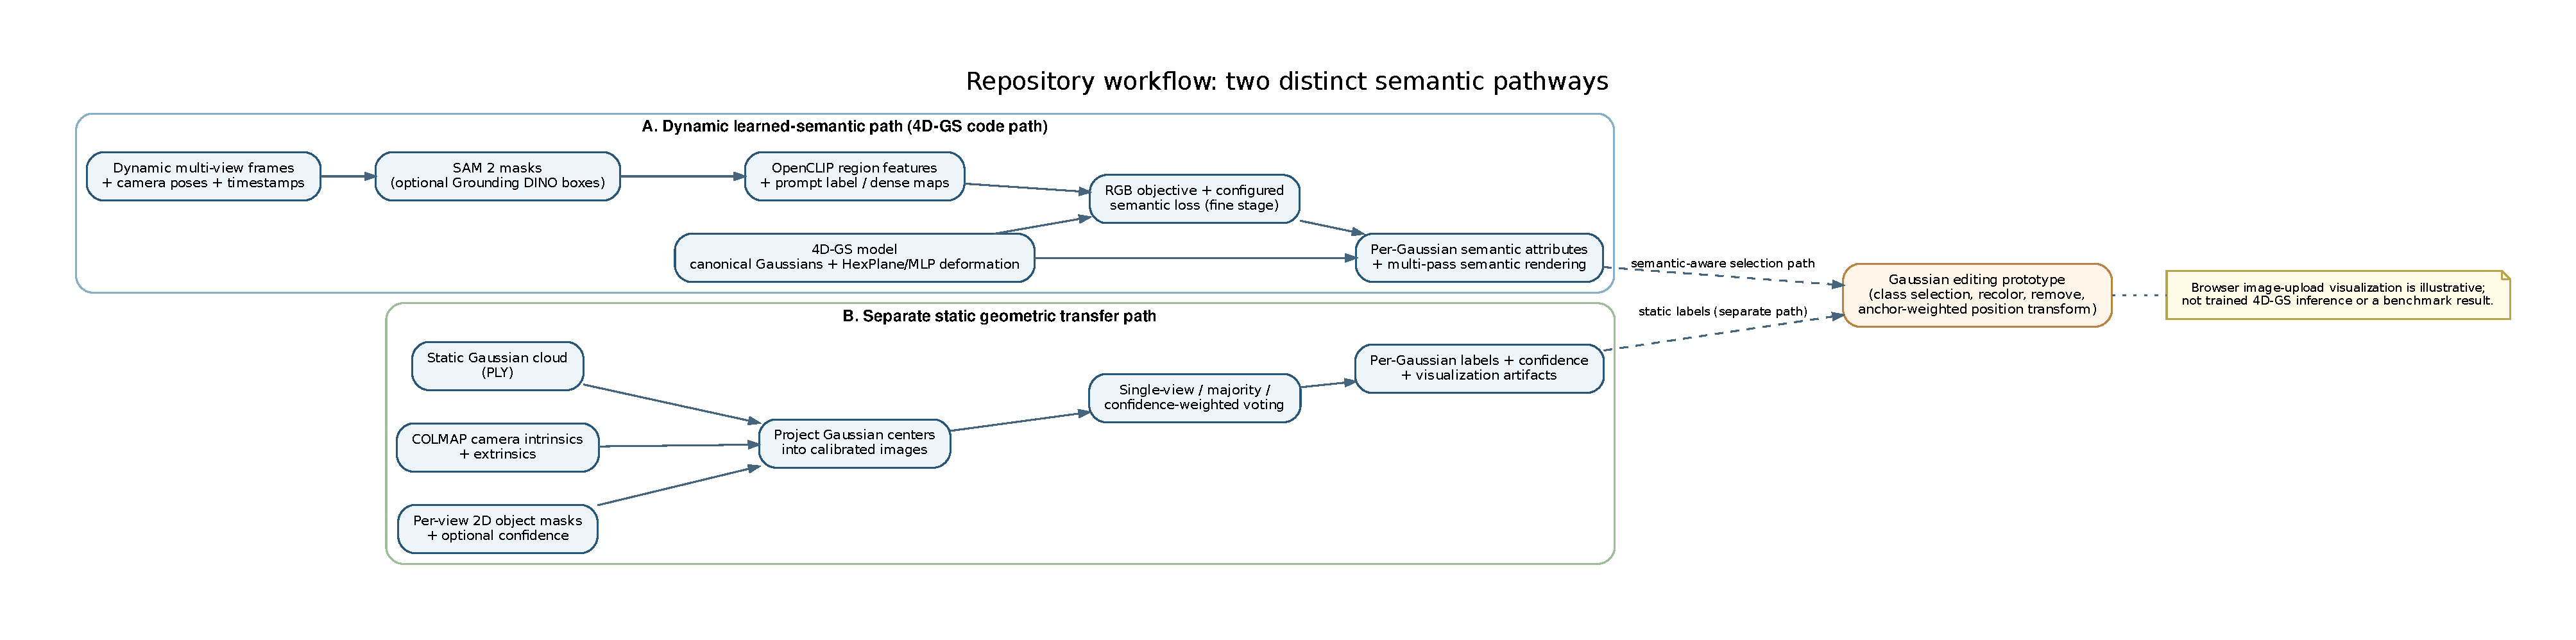
\includegraphics[width=0.98\textwidth]{workflow_diagram.pdf}
\caption{Repository workflow, reconstructed from the code paths. The dynamic semantic-training pathway and the static projection/voting pathway are distinct. Dashed editor links describe available prototype operations, not a verified end-to-end trained dynamic editing demonstration.}
\label{fig:pipeline}
\end{figure*}

\section{Method}
\subsection{Dynamic Gaussian Representation}
The dynamic model starts from canonical Gaussian primitives with means $\boldsymbol{\mu}_i$, positive scales $\mathbf{s}_i$, rotations $R_i$, opacity $o_i$, and appearance coefficients. A covariance may be written as
\begin{equation}
\Sigma_i=R_i\operatorname{diag}(\mathbf{s}_i^2)R_i^{\mathsf T}.
\end{equation}
At timestamp $t$, the deformation network predicts parameter offsets; for position, $\boldsymbol{\mu}_i(t)=\boldsymbol{\mu}_i+\Delta\boldsymbol{\mu}_i(t)$. The repository uses a HexPlane feature field and a lightweight MLP in this deformation path~\cite{wu20244dgs,wang2023hexplane}. The differentiable splatting renderer alpha-composites ordered Gaussian contributions; for RGB color $\mathbf{c}_i(t)$,
\begin{equation}
\mathbf{C}(p,t)=\sum_i T_i(p,t)\alpha_i(p,t)\mathbf{c}_i(t),\qquad
T_i(p,t)=\prod_{j<i}\left(1-\alpha_j(p,t)\right).
\end{equation}
This notation summarizes the rendering formulation; this report does not assert a newly proposed deformation architecture.

\subsection{2D Semantic Target Construction}
For each input frame, the preprocessing pipeline obtains masks from SAM 2; an optional Grounding DINO stage can provide text-conditioned boxes before SAM 2 segmentation. CLIP image features are extracted for masked image crops. Given normalized image feature $\mathbf{f}_i$ for region $i$ and normalized text features $\mathbf{t}_k$ for prompts $k$, the implementation assigns a prompt label by maximum cosine similarity:
\begin{equation}
\hat{k}_i = \arg\max_k \; \mathbf{f}_i^{\mathsf T}\mathbf{t}_k.
\end{equation}
Mask labels are composed into a per-pixel label map, reserving label zero for unlabeled/background pixels. Dense feature maps assign each pixel the feature of its associated mask; pixels outside masks receive a zero vector. These are model-generated pseudo-targets and may contain segmentation, association, and prompt-classification errors.

If $M_i(p)\in\{0,1\}$ indicates membership of pixel $p$ in region $i$, the stored label map is composed from the prompt assignment of the selected mask, with background index zero reserved for unlabeled pixels. The implementation resolves overlapping masks according to the mask ordering/quality metadata; it does not estimate an independent ground-truth 3D label.

\subsection{Semantic Attributes in the Dynamic Gaussian Model}
The Gaussian model can allocate a trainable semantic vector $\mathbf{s}_j$ for each Gaussian $j$ when semantic features are enabled. A semantic rasterizer renders these attributes using the scene's visibility and opacity contributions. In conceptual form, the rendered semantic feature at pixel $p$ is
\begin{equation}
\mathbf{S}(p,t) = \sum_j T_j(p,t)\,\alpha_j(p,t)\,\mathbf{s}_j,
\end{equation}
where $T_j$ is accumulated transmittance before Gaussian $j$ and $\alpha_j$ is its pixel contribution. In the usual front-to-back compositing notation, $T_j=\prod_{m<j}(1-\alpha_m)$; this expression describes the rasterizer's semantic compositing, not a separate semantic opacity model. The implementation reuses the camera, deformation, opacity, scale, and rotation path used by RGB rendering and divides $D$ feature channels into groups of at most three for rasterizer passes.

The RGB objective combines an $\ell_1$ reconstruction term and an optional DSSIM term. During fine-stage semantic training, the implementation loads label and/or feature supervision for a camera frame and adds the configured semantic objective. For a label map $Y$ and rendered class logits $Z$, the cross-entropy path ignores label zero:
\begin{equation}
\mathcal{L}_{\mathrm{CE}}=-\frac{1}{|\Omega|}\sum_{p\in\Omega}\log\frac{\exp Z_{Y_p}(p)}{\sum_{c=1}^{K}\exp Z_c(p)}, \qquad \Omega=\{p:Y_p\ne 0\}.
\end{equation}
For normalized rendered feature $\hat{F}_p$ and target feature $\hat{G}_p$, the cosine mode uses $\mathcal{L}_{\cos}=1-|\Omega|^{-1}\sum_{p\in\Omega}\hat{F}_p^{\mathsf T}\hat{G}_p$; the MSE mode compares feature maps elementwise. The RGB and semantic objectives are combined as
\begin{equation}
\mathcal{L}_{\mathrm{RGB}}=\mathcal{L}_{1}+\lambda_{\mathrm{DSSIM}}(1-\mathrm{SSIM}),\qquad
\mathcal{L}_{\mathrm{total}}=\mathcal{L}_{\mathrm{RGB}}+\lambda_{\mathrm{sem}}\mathcal{L}_{\mathrm{sem}}.
\end{equation}
The configured semantic mode is cross-entropy for label maps or cosine/MSE for feature maps. The training hook accumulates valid-camera semantic losses and averages them before applying $\lambda_{\mathrm{sem}}$. Exact behavior depends on configuration and target availability. The code does not by itself establish that a particular trained checkpoint was produced successfully.

\subsection{Static Multi-View Projection and Voting}
For a static Gaussian center $\mathbf{X}_w$, the pipeline transforms it into camera coordinates by $\mathbf{X}_c=R\mathbf{X}_w+\mathbf{t}$ and applies pinhole projection. For camera intrinsics $(f_x,f_y,c_x,c_y)$ and camera-space point $(X_c,Y_c,Z_c)$ with $Z_c>0$,
\begin{equation}
 u=f_x X_c/Z_c+c_x, \qquad v=f_y Y_c/Z_c+c_y.
\end{equation}
Points behind the camera or outside the image bounds are excluded. The projected pixel is sampled in the corresponding binary/object mask to generate a per-view vote $v_{gc}$ for Gaussian $g$ in camera $c$; $v_{gc}=-1$ denotes no vote. The single-view baseline uses the most informative view $c^*=\arg\max_c\sum_g\mathbf{1}[v_{gc}\ne -1]$. Equal-weight majority voting uses $\hat{y}_g=\arg\max_k\sum_c\mathbf{1}[v_{gc}=k]$, with unsupported Gaussians kept unknown. For the confidence-weighted variant, the implementation uses mask confidence $q_{gc}$, normalized camera distance $d_{gc}$, and optionally mean Gaussian scale $s_g$:
\begin{equation}
w_{gc}=q_{gc}\frac{1}{1+d_{gc}/(\operatorname{median}(d)+\epsilon)}\,\operatorname{clip}\!\left(\frac{s_g}{\operatorname{median}(s)+\epsilon},0.1,3\right),
\end{equation}
where the scale factor is one when scale information is unavailable. It selects $\hat{y}_g=\arg\max_k\sum_{c:v_{gc}=k}w_{gc}$ and reports confidence as the winning weight divided by total observed weight. A configured minimum-view constraint leaves insufficiently supported points unknown. The code implements these voting strategies; ablation execution still requires actual matching camera, mask, and trained static-Gaussian artifacts. This is geometric label transfer for a static cloud, not a metric of dynamic 4D semantic reconstruction.

\subsection{Prototype Gaussian Editing}
The editor can select Gaussians by class logits, recolor the DC spherical-harmonic appearance coefficient, reduce opacity for removal/isolation, and transform selected positions. For selected points $x_i$ and anchors $a_j$, the current skinning weights are
\begin{equation}
w_{ij}=\frac{\exp(-\|x_i-a_j\|^2/(2\sigma^2))}{\sum_l\exp(-\|x_i-a_l\|^2/(2\sigma^2))},\qquad
x_i'=\sum_j w_{ij}\,T_j(x_i),
\end{equation}
with anchors selected by farthest-point sampling and $\sigma^2$ derived from the mean squared anchor distance. This does not optimize an ARAP energy, and the present behavior should not be interpreted as verified physical deformation. Covariance/orientation and consistency through the learned temporal deformation require further implementation and testing.

\section{Implementation}
The codebase is organized around the upstream 4D-GS model/training/rendering structure, with project additions in the preprocessing, semantic loading, rendering, evaluation, integration, and editing modules. Table~\ref{tab:status} summarizes what is available and the evidence boundary.

\subsection{Execution and Artifact Flow}
The dynamic path expects a prepared dynamic scene with frame names, timestamps, and camera metadata; D-NeRF is one source of synthetic dynamic-scene data in the project workflow~\cite{pumarolaDNeRF2021}. Semantic extraction writes per-frame masks, integer label images, feature maps, and metadata. The semantic loader matches frame names to these artifacts, and the training hook applies the configured semantic objective during fine-stage iterations when suitable targets are available. Semantic feature rendering uses rasterizer passes of up to three channels. The static integration path instead expects a trained static Gaussian PLY, a COLMAP dataset with matching image names, and masks for those views; its CLI writes Gaussian labels, confidence, previews, top-down visualizations, and run metrics. These filesystem contracts are necessary for reproducibility and clarify that the static path is not an evaluation of the dynamic path.

\begin{table}[t]
\caption{Implementation status and evidence boundary}
\label{tab:status}
\centering
\footnotesize
\begin{tabular}{p{0.27\columnwidth}p{0.28\columnwidth}p{0.37\columnwidth}}
\toprule
Component & Repository evidence & What remains unverified \\
\midrule
4D-GS baseline & Training, deformation, and render code paths & Reproduction logs, checkpoint, and matched benchmark run \\
SAM 2--CLIP & Mask, feature, and prompt-label extraction modules & Target quality and cross-frame identity stability \\
Dynamic semantic path & Semantic attributes, loader, loss and render hooks & Held-out semantic accuracy and temporal consistency \\
Static voting path & Calibrated projection and three voting strategies & Accuracy against independent labeled 3D/2D ground truth \\
Editing prototype & Class selection and Gaussian appearance/position operations & 4D coherence, covariance handling, and true ARAP optimization \\
Browser upload demo & Image-dependent synthetic point visualization & No learned reconstruction or model inference \\
\bottomrule
\end{tabular}
\end{table}

\subsection{Qualitative Visualization}
Fig.~\ref{fig:qualitative} shows an existing repository RGB/semantic comparison asset. It documents the intended visualization only: no source checkpoint, render manifest, camera/time split, or manual annotation is archived alongside it. Accordingly, it is not evidence of a trained run or an evaluated test result.

\begin{figure}[t]
\centering
\includegraphics[width=0.98\columnwidth]{demo_semantic_comparison.png}
\caption{Repository RGB/semantic comparison asset. The figure is qualitative and its checkpoint provenance is unavailable; it is included to illustrate the intended output format, not as a measured result.}
\label{fig:qualitative}
\end{figure}

\section{Experimental Protocol and Current Results}
\subsection{Metrics}
For predicted label map $P$ and independent ground-truth map $G$, the pixel-space intersection-over-union for class $k$ is
\begin{equation}
\operatorname{IoU}_k=\frac{|\{p:P_p=k\}\cap\{p:G_p=k\}|}{|\{p:P_p=k\}\cup\{p:G_p=k\}|},\qquad
\operatorname{mIoU}=\frac{1}{|\mathcal{K}|}\sum_{k\in\mathcal{K}}\operatorname{IoU}_k.
\end{equation}
The checked-in evaluator matches single-channel PNGs by filename, verifies shape and class range, excludes background index zero, and averages classes with nonzero union. This measures 2D label-map agreement only, not 3D semantic accuracy. For a future held-out RGB evaluation, PSNR would use $10\log_{10}(L^2/\mathrm{MSE})$ with the image peak range $L$ stated; SSIM must also report its implementation and settings~\cite{wangSSIM2004}. The checked-in evaluator does not produce PSNR, SSIM, LPIPS, FPS, temporal correspondence, or edit-quality metrics. Temporal consistency must use valid correspondences such as known synthetic correspondences or projected Gaussian identities; same-pixel adjacent-frame agreement is invalid when objects move.

\subsection{Ablation Design and Execution Status}
The static projection program implements the first three variants below and provides an ablation runner. The repository does not contain the matching trained static PLY, COLMAP scene, and mask artifacts needed to run that comparison, so all outcome cells are explicitly marked not run. Dynamic variants below are a proposed controlled evaluation based on the existing semantic loss hooks; a correspondence-consistency training loss is not implemented and is included only as future work.

\begin{table*}[t]
\caption{Ablation plan and evidence status. ``Not run'' means no valid scene-level outputs are archived.}
\label{tab:ablations}
\centering
\footnotesize
\begin{tabularx}{\textwidth}{p{0.18\textwidth}p{0.28\textwidth}p{0.18\textwidth}X}
\toprule
Path & Variant & Code status & Result / required measurement \\
\midrule
Static projection & Most-informative single view & Implemented & Not run; compare coverage and label agreement on a fixed Gaussian set \\
Static projection & Equal-weight majority & Implemented & Not run; report coverage and per-class IoU against independent labels \\
Static projection & Confidence-weighted voting & Implemented & Not run; compare with majority on identical views, masks, and Gaussians \\
Dynamic semantics & RGB-only 4D-GS & Baseline path present & No verified checkpoint archived; measure held-out PSNR/SSIM and runtime \\
Dynamic semantics & Label supervision (cross-entropy) & Loss path present & Not run as a controlled ablation; measure held-out pixel mIoU \\
Dynamic semantics & CLIP feature supervision (cosine/MSE) & Loss paths present & Not run as a controlled ablation; measure held-out feature and label agreement \\
Dynamic semantics & Label-target vs. CLIP-feature-target runs & Separate configurable loss modes & Not run as a controlled comparison; hold scene, initialization, views, and schedule fixed \\
Temporal consistency & Correspondence-consistency loss & Not implemented & Future experiment only; not a current method or result \\
\bottomrule
\end{tabularx}
\end{table*}

\subsection{Current Evidence and Results}
The repository has no archived held-out semantic predictions with independent ground truth, and no traceable dynamic training run/checkpoint for this report. Former draft values for mIoU, temporal consistency, PSNR, SSIM, FPS, and editing latency are therefore withdrawn and omitted. As a software check, the available CPU-oriented tests were run with the semantic-editing test module excluded: 41 passed and one COLMAP text-model test failed because the official Gaussian-Splatting submodule loader is absent. The semantic-editing test module itself could not be collected in the selected virtual environment because PyTorch is not installed. These unit tests do not validate scene-level reconstruction quality.

\begin{table}[t]
\caption{Results evidence available at report preparation}
\label{tab:results}
\centering
\footnotesize
\begin{tabular}{p{0.37\columnwidth}p{0.47\columnwidth}}
\toprule
Measure / artifact & Evidence-based status \\
\midrule
Dynamic checkpoint and training logs & No reproducible run archived \\
Held-out semantic predictions and manual labels & Not available; mIoU not reported \\
PSNR / SSIM / LPIPS & Not measured by checked-in evaluator \\
Temporal correspondence metric & Not implemented or measured \\
Render FPS / memory / edit latency & No reproducible measurement record \\
Static voting ablation & Runner exists; required scene artifacts/results absent \\
CPU integration test subset & 41 passed; one blocked by missing upstream loader; editor test requires PyTorch \\
RGB/semantic figure & Qualitative repository asset only; caveat in Fig.~\ref{fig:qualitative} \\
\bottomrule
\end{tabular}
\end{table}

\subsection{Reproducible Evaluation Protocol}
A valid experiment should archive the scene, camera and timestamp split, class mapping and prompts, configuration, checkpoint, hardware/software versions, command line, rendered predictions, independent labels, and machine-readable metrics. Baseline and semantic models must use matched data, resolution, views, timestamps, and hardware. For the static voting ablation, hold the Gaussian cloud, cameras, and masks fixed across one-view, majority, and weighted variants. Report per-class and macro IoU on held-out manual labels; evaluate temporal labels only on known correspondences; and report synchronized warm-up and timed costs separately for RGB rendering, semantic rendering, preprocessing, and editing. These are required experiments, not results asserted by this paper.

\subsection{Limitations}
The semantic targets inherit errors from the segmentation model, prompt design, mask overlap, and occlusion. Per-frame region labels do not guarantee persistent object identity. The static projection pipeline assumes known camera calibration and a static cloud, and point-center sampling may be sensitive to rasterization and visibility boundaries. The editing prototype modifies Gaussian parameters but does not yet demonstrate temporally coherent physical edits or a true ARAP solve. Finally, the browser upload visualization is illustrative and should not be presented as trained model output.

\section{Conclusion}
This report documents a prototype for adding semantic supervision and editing interfaces around dynamic Gaussian splatting. The repository contains a dynamic learned-semantic path, a separate static geometric multi-view transfer pipeline, and a Gaussian editing prototype. These are useful foundations for experimentation, but source-code presence is not equivalent to a reproduced end-to-end result. The next research step is to run a fixed scene and held-out evaluation with archived checkpoints and labels, then measure semantic accuracy, temporal consistency, visual quality, efficiency, and edit coherence under controlled conditions.

\bibliographystyle{IEEEtran}
\bibliography{references}
\end{document}
